\hyphenation{de-mon-stra-te}
\hyphenation{trans-act-ion}

\newcommand{\uniform}[1]{\mathcal{U}_{#1}}
\newcommand{\set}[1]{\left\lbrace #1 \right\rbrace}

\section{Evaluation}
\label{sec:eval}

We evaluate Mediator on a distributed testbed, and assess the system 
performance (throughput and latency) metrics, as well as the ratio of 
aborted transactions. The latter is an upper bound on the ratio of false
aborts, which captures system's negative impact on client applications,
and is expected to be low. We experiment with multiple workloads 
that feature different traffic mixes (varying proportions of gets 
versus puts, transactional versus native operations) and different
distributions of transaction size (single-access versus bulk transactions). 
Mediator's behavior is explored in the context of snapshot isolation
and serializability models. 

We compare a system in which transactions are served by Mediator 
and native traffic is handled by HBase with a system in which native
operations are transactified, and all the traffic is served by Omid. For 
brevity, we call the first system Mediator and the second system Omid. 

We start by analyzing the overhead transaction processing imposes 
on native operations. Following this, we study Mediator's impact on the 
{\em overall} system throughput. Namely, we explore Mediator's and Omid's  
{\em comfort zones\/} --  the workload patterns for which one platform 
performs significantly better than its counterpart. 

\setlength{\abovecaptionskip}{7pt}
\setlength{\belowcaptionskip}{-2pt}
\begin{figure*}[ht]

  \centering {
	\begin{subfigure}[b]{0.33\textwidth}
		{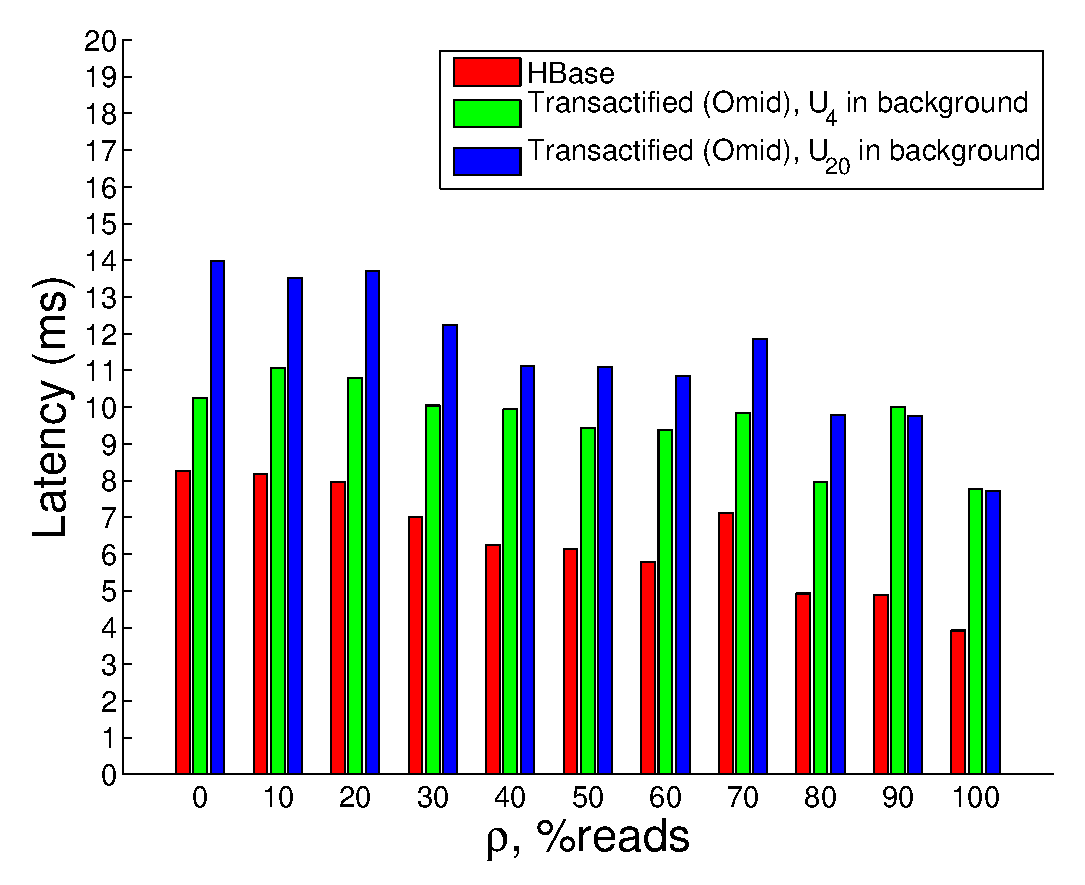
\includegraphics[width=2in]{Figs/matlab/omid_native_latency_u19_10n.eps}}
		\caption{$\uniform{1}$ workload ($\uniform{4}$, $\uniform{20}$ in the background).}
	\end{subfigure}
\quad
  \begin{subfigure}[b]{0.3\textwidth}
		{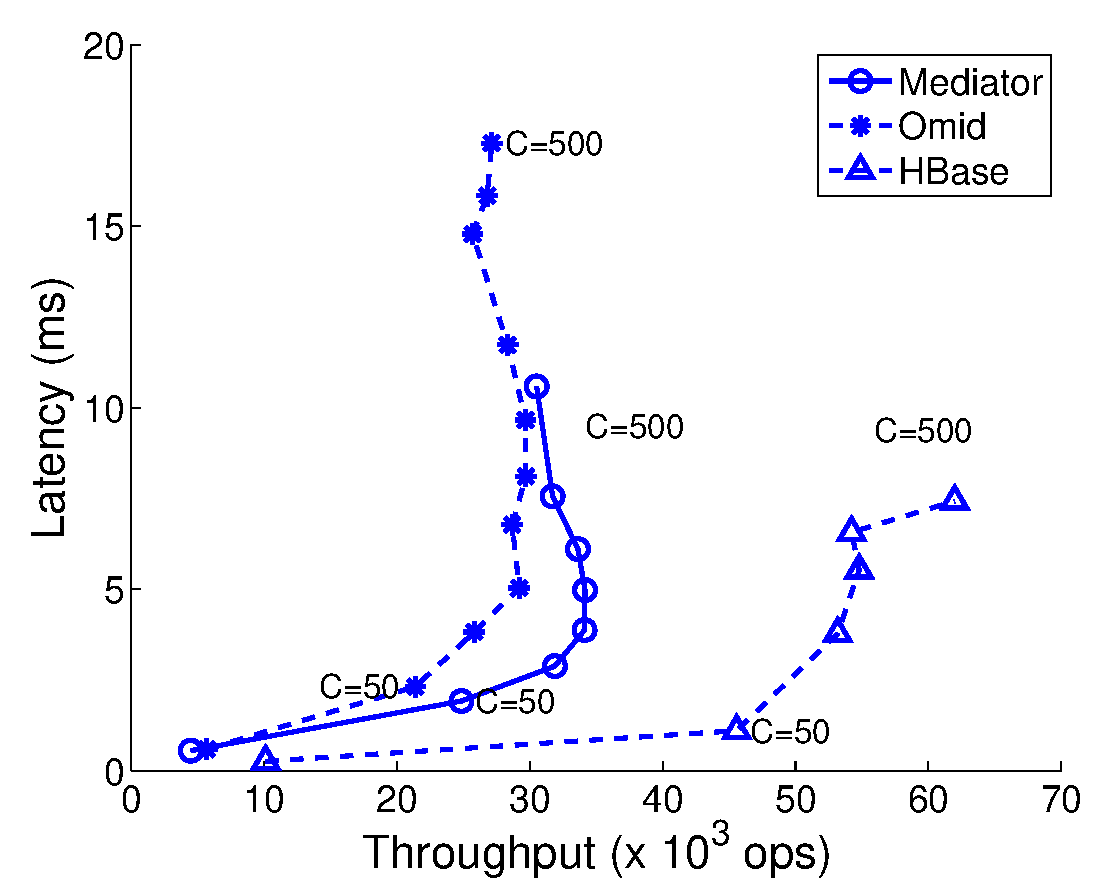
\includegraphics[width=2in]{Figs/matlab/throughput_latency_u1_90r.eps}}
		\caption{Read-dominated $\uniform{1}$ workload.}
  \end{subfigure}%
  \quad
	\begin{subfigure}[b]{0.3\textwidth}
		{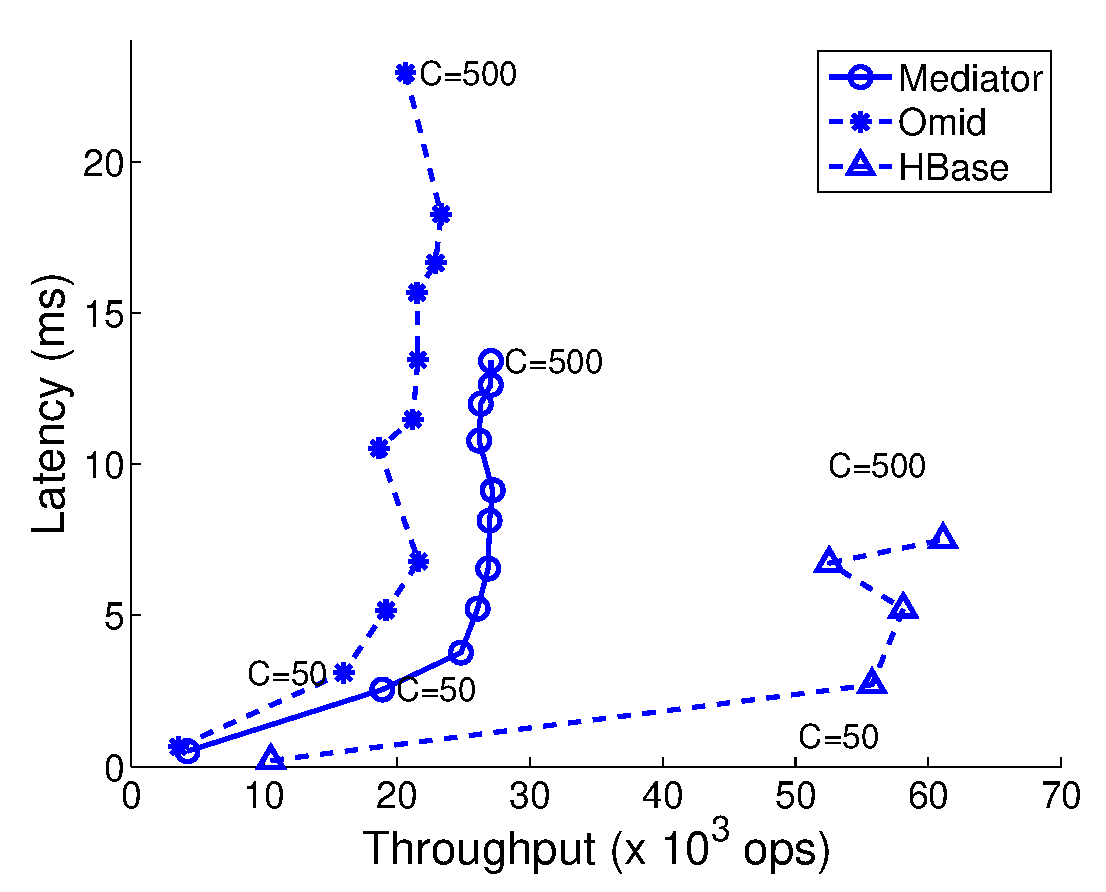
\includegraphics[width=2in]{Figs/matlab/throughput_latency_u1_50r.eps}}
		\caption{Write-intensive $\uniform{1}$ workload.}
	\end{subfigure}
}
\caption{\bf{\small{Transaction processing's performance overhead on gets and puts. 
(a) Latency perspective. HBase compared to Omid's single-operation ($\uniform{1}$) transactions, with larger transactions in the background. 
Fixed number of clients ($C=200$), running read ratio ($0 \leq \rho \leq 1$).
(b,c) Throughput-Latency perspective. HBase compared to Omid's and Mediator's $\uniform{1}$ transactions. 
Running number of clients ($5 \leq C \leq 500$).} }}

\label{fig:txn_only_si}
%\vskip -.2.5in
\end{figure*}

\subsection{Environment}
\label{sec:testing platform}

We utilize a cluster of machines equipped with a $4$-core $2.50$ GHz Xeon(R) L5420 
CPU and $16$ GB RAM. All services are implemented in Java, with the JVM using $4$ GB heap.  
Separate nodes are allocated to the datababse ($10$), the log ($10$),  the TSO ($1$), and the clients ($20$). 

The key-value store is HBase, deployed on top of Hadoop's distributed filesystem, HDFS, with a replication 
factor of $3$. The HBase database (region) servers are co-located with HDFS storage servers (datanodes) for 
efficiency. The dataset under test holds $200$ million records. Each record
is 1 KB long, with a 12 bytes long key. That is, the database's size is
approximately $200$ GB, each server controlling $10\%$ thereof.  The block cache at each server defaults to $40\%$
of the heap.

%In order to explore the settings in which transaction processing introduces a
% meaningful overhead, 
We are interested in latency-oriented applications and therefore focus on
configurations that serve individual operations with low latency.
We address workloads with reasonable locality of gets -- the keys are drawn from
a Zipfian distribution that generates approximately a $90\%$ cache hit rate. The
put latencies are insensitive to key distribution since HBase servers employs
LSM trees~\cite{FDPlus2012} that absorb multiple writes into a memory buffer.
To keep the changes to the database layer minimal, we do not try to optimize the HBase overhead 
by switching off the database's internal write-ahead logging (which is redundant with Mediator's log 
for transactional traffic).
 
We perform a large set of experiments on a variety of workloads. A single experiment performs 
$500{,}000$ gets and puts. Each client node concurrently drives the system's workload through 
up to $40$ concurrent processes of YCSB~\cite{YCSB2010}, a popular load generator. 
The YCSB clients exercise the Mediator, Omid, and HBase API's, depending on the configuration. 

In a single experiment, each YCSB instance drives the same traffic pattern, therefore the cumulative 
workload remains steady over time. In other words, each client generates the same load bandwidth, 
which splits independently among (1) reads and writes, and (2) transactional and native accesses. 
We denote the fraction of reads by $\rho$, and the fraction of native operations by $\nu$. 
In the Omid setting, YCSB transactifies all the original native operations. In both settings, 
transactional accesses are clustered in transactions of varying sizes, picked 
uniformly at random from a range $[1, 2, \ldots, n]$, where $n$ is specified by the 
experiment. We denote this distribution $\uniform{n}$. The larger $n$ is, the wider the spectrum 
of the exercised transaction sizes is -- from a single access to a bulk of operations. 
$\uniform{1}$ is a non-realistic workload (singleton transactions workload is
meaningless) that we use to demonstrate the local-commit optimization. Table~\ref{tab:notation} 
summarizes the notation. 

Mediator log is implemented through Bookkeeper~\cite{Bookkeeper2013}. 
Finally, the TSO employs $1024$-bits-wide Bloom filters.

\setlength{\belowcaptionskip}{0pt}
\setlength{\abovecaptionskip}{6pt}
\begin{table} [t]
\small{
%\hrulefill
\begin{tabular}{lll}
{\bf Notation} & {\bf Description} & {\bf Values} \\
\hline
$C$ & number of concurrent clients & $50, 100, \ldots, 1200$ \\
$\nu$ & ratio of native operations & $0, 0.1, \ldots, 1$ \\
$\rho$ & ratio of get accesses & $0, 0.1, \ldots, 1$  \\
$\uniform{n}$ & transaction size distribution & $\uniform{1}$ (singletons), \\
& (uniform over $[1, 2, \ldots n]$) & $\uniform{4}$, $\uniform{20}$
\end{tabular}
}
%\vskip .1in
\caption{\bf{\small{Workload parameter notation.}}}
\label{tab:notation}
%\vskip -.2.5in
\end{table}

\subsection{Numerical Results -- Snapshot Isolation}
\label{sec:tests:si}

This section studies Mediator's performance under the snapshot isolation consistency model. 

\begin{figure*}
  \centering
  \begin{subfigure}[t]{0.3\textwidth}
   %\flushleft
   \center
		{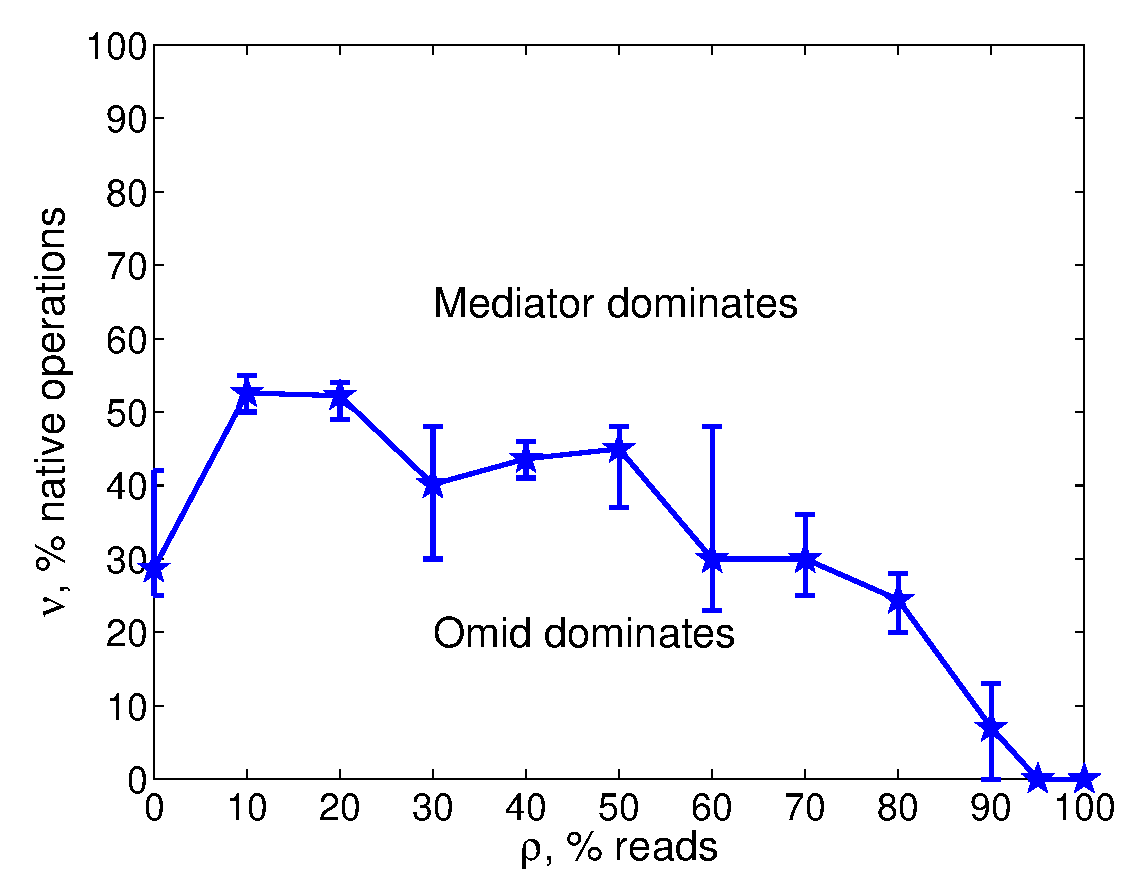
\includegraphics[width=2in]{Figs/matlab/equilibrium_curve_u4.eps}}
		\caption{Equilibrium curve for $\uniform{4}$.}
               \label{fig:heatmap}
  \end{subfigure}%
%\hspace{0.4in}
\quad
	\begin{subfigure}[t]{0.3\textwidth}
		{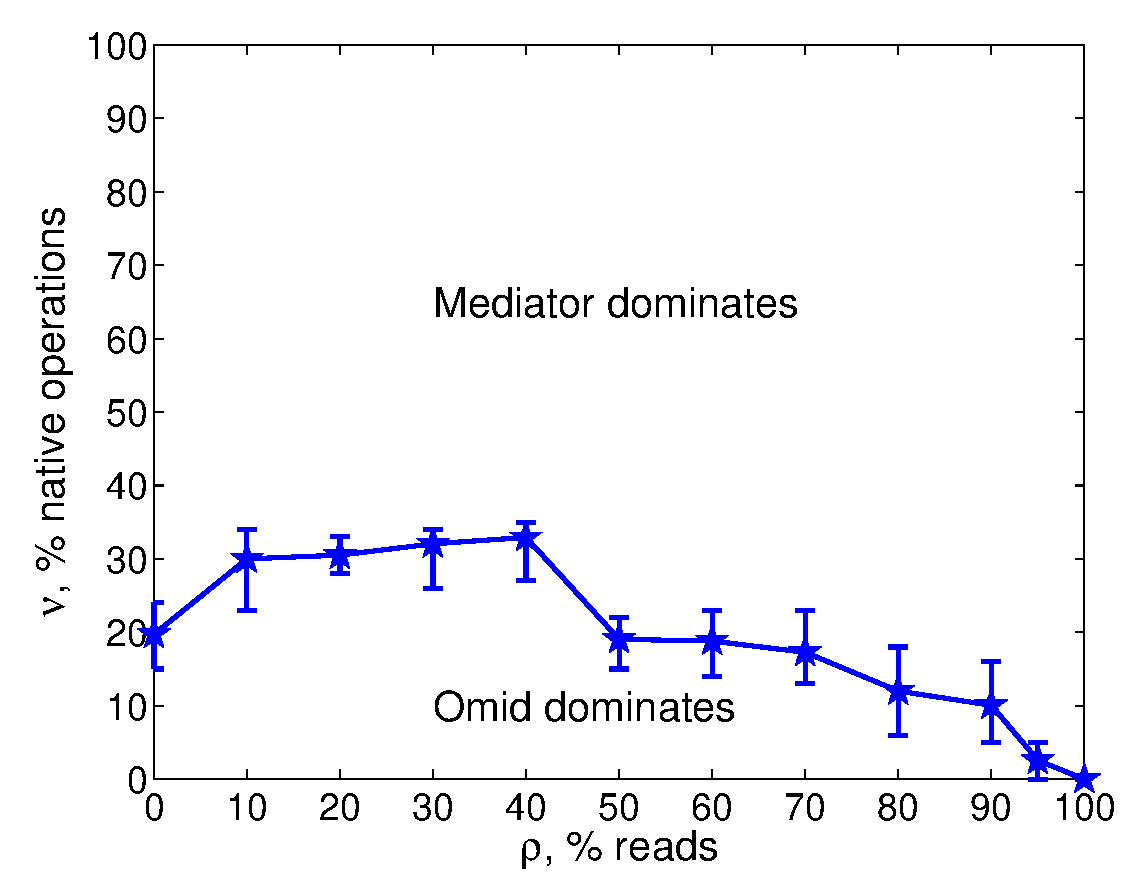
\includegraphics[width=2in]{Figs/matlab/equilibrium_curve_u19.eps}}
		\caption{Equilibrium curve for  $\uniform{20}$.}
       \label{fig:curves}
       \end{subfigure}
\quad
       \begin{subfigure}[t]{0.3\textwidth}
	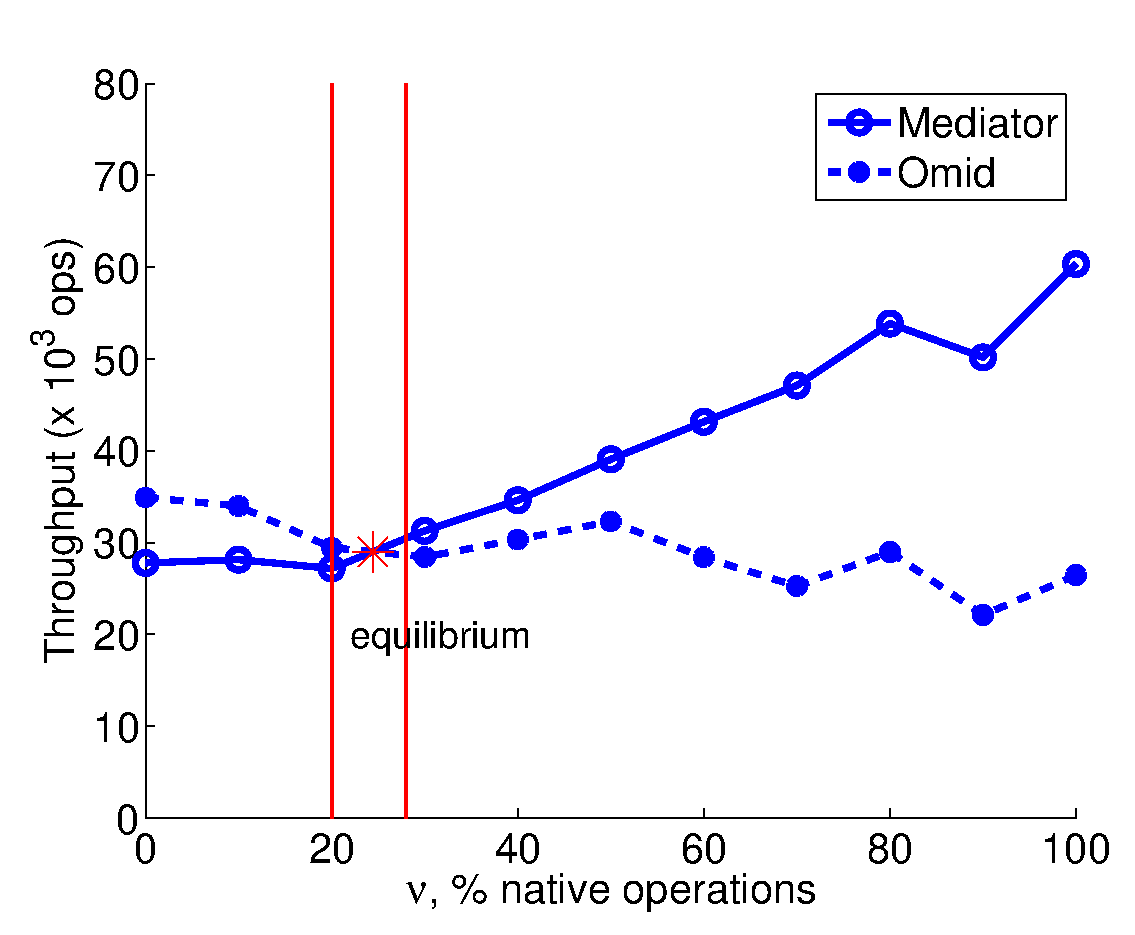
\includegraphics[width=2in]{Figs/matlab/equilibrium_90r_u4.eps}
	\caption{An equilibrium point, $\uniform{4}$, $\rho=0.8$.}
	\end{subfigure}

\caption{\bf{\small{Comfort zones of Mediator and Omid, for a variety of read-write mixes ($0 \leq \rho \leq 1$) 
and transactional-native mixes ($0 \leq \nu \leq 1$). The workload is generated by $200$ clients.
}}}
\label{fig:equilibrium}
\end{figure*}

{\bf Latency Overhead on Single Operations.} 
We start by motivating the advantage of serving native traffic directly. 
Our first experiment demonstrates the surplus to the median latency of native HBase operations 
when the latter are transactified with Omid. We consider three configurations: (1) 100\% native traffic, 
(2) single-operation ($\uniform{1}$) transactions with background $\uniform{4}$ traffic, and 
(3) the same with background $\uniform{20}$ traffic. The workload is driven by 200 clients. 
We explore a variety of read ratios ($0 \leq \rho \leq 1$). 

Figure~\ref{fig:txn_only_si}(a) shows the results. The penalty grows with the fraction of writes
and the background transactions' bulkiness. This is explained as follows. Transactions introduce 
a fixed communication overhead (round trip upon begin and commit), and the TSO state replication 
overhead. The TSO state depends on the number of keys updated by individual transactions, 
i.e., for the same read/write ratio the larger transactions populate a larger state, which translates
to a larger replication overhead, and eventually to larger latencies incurred to short transactions. 
For example, in write-only workloads in which transactified puts run in parallel with $\uniform{20}$ 
transactions, the put latency becomes almost twice as large as that of the native HBase operation.   

The next example provides a different perspective on the same phenomenon. We compare the median
operation latency and the system throughput for the traffic of $100\%$ single operations ($\uniform{1}$), 
in the following scenarios: (1) native operations, (2) the same, transactified with Omid, and (3) the same, 
transactified with Mediator. We observe the performance for varying numbers of clients, and draw the 
throughput-latency curves. All implementations are considered in two settings -- a read-dominated workload 
($\rho=0.9$, Figure~\ref{fig:txn_only_si}(b)), and a write-intensive workload ($\rho=0.5$, Figure~\ref{fig:txn_only_si}(c)). 
We see that even without any bulky transactions in the background, Omid and Mediator are inferior to
bare-metal HBase. For example, Mediator scales to approximately $35$K operations per second (ops) 
in the read-dominated scenario, and to $28$K in the write-intensive one, whereas HBase achieves above 
$55$K ops\footnote{\footnotesize{The same HBase configuration scores much higher throughputs 
for bulk I/O. This setting is not the focus of our experiment.}}. These results emphasize the potential 
of consolidating transactional and non-transactional traffic within the same framework, 
to avoid the overhead of transactifying the latter.

% Face-off!
%\subsubsection{Mixed Traffic} 
%\label{sec:tests:si:mixed}

{\bf Total Throughput.} 
We now turn to our main goal -- contrasting Mediator with Omid on a wide variety of mixed workloads. 
We study the $\uniform{1}$, $\uniform{4}$ and $\uniform{20}$  distributions.   

The $\uniform{1}$ case is an exception -- Mediator is faster than Omid in all configurations
(Figure~\ref{fig:txn_only_si}(b) and Figure~\ref{fig:txn_only_si}(c) demonstrate this for two
specific cases). This happens by the virtue of its no-commit optimization (which
serves single-get transactions) and its local-update optimization (which serves
single-put transactions). Either way, Mediator client does not communicate with
the TSO upon commit skipping consistency checks and logging, hence, the oracle's
state remains void. Upon transaction begin, the state replicated to the client 
is minimal (transaction timestamp), and therefore Mediator's overhead is smaller. Obviously,
if Mediator is faster for all-transactional $\uniform{1}$ traffic, the same holds if part of the workload
is native. 

The comparison becomes interesting for truly mixed workloads, in which native operations
run side by side with transactions of different sizes. Both Omid and Mediator have their strong points.
The former is superior for transactional traffic, since it avoids the WAL overhead (Section~\ref{sec:overview}). 
The latter is faster for native traffic. In this context, the cumulative throughput (in terms of both transactional 
and native operations) is a convenient metric for evaluating the overall system performance. (Note that in 
an environment in which get and put operations are clustered in transactions,
the latency of individual operations is not well-defined.) 

The following experiment employs $200$ clients, and exercises all combinations of read ratios 
($0 \leq \rho \leq 1$) and native access ratios ($0 \leq \nu \leq 1$). In this context, for a given 
read ratio $\rho$, an {\em equilibrium point\/} is the smallest ratio of native operations $\nu$ 
for which Mediator achieves a larger throughput. The collection of equilibrium points for a given 
workload type defines an {\em equilibrium curve}. This curve separates Mediator's and Omid's 
comfort zones. The area above it is the fraction of configurations in which Mediator 
is superior. 

Figure~\ref{fig:equilibrium}(a) and Figure~\ref{fig:equilibrium}(b) portray the equilibrium curves 
for $\uniform{4}$ and $\uniform{20}$, respectively. Every data point is depicted with a $10\%$
confidence interval. Mediator outperforms Omid in a vast majority of configurations -- in particular, 
in any read-write mix with $\nu \geq 50\%$. It is consistently more advantageous for $\uniform{20}$ 
versus $\uniform{4}$, due a better manifestation of write batching in bulk transactions. For both workloads, 
Mediator's dominance is more pronounced for the extreme values of $\rho$. For example, for $\rho=1$, 
the no-commit optimization applies to all transactions, thus reducing the equilibrium point to zero; 
for $\rho=0$, the local-commit optimization applies to singleton transactions
(only part of the workload).

\remove{
Figure~\ref{fig:equilibrium}(b) zooms in on the results from Figure~\ref{fig:equilibrium}(a).
The throughput ratio between Mediator and Omid for the $\uniform{4}$ distribution is depicted 
in a log-scale ``heat map'' presentation. The areas in which Mediator prevails appear in warm 
tones. The zero-isoheight boundary (marked by $\Diamond$) captures the equilibrium curve. 
Note that the absolute performance gaps are bigger in Mediator's dominance area. 
}

Figure~\ref{fig:equilibrium}(c) zooms in on how a single equilibrium point is computed.
For a given read ratio $\rho$, Mediator's throughput monotonically increases with the 
fraction of native traffic $\nu$ (which is natural, since the latter has no overhead). 
On the contrary, Omid's throughput does not grow with $\nu$. This happens because 
the system wraps every individual access as a transaction. For non-singleton 
transactions ($\uniform{4}$ and $\uniform{20}$), the overhead grows disproportionately 
with $\nu$, thus reducing the total throughput. The crossing of the two curves is an equilibrium 
point; the vertical bars mark the areas of statistically significant dominance. 

%\subsubsection{Abort Ratio}
%\label{sec:tests:si:abort_ratio}

{\bf Abort Ratio.} 
We explore the {\em abort ratios\/} incurred by Mediator to user applications --
i.e., the fraction of transactios that get aborted due to (possibly falsely) 	
detected conflicts.  The probability of colliding with concurrent operations grows 
with the fraction of updates and with the transaction size. The 
computation of the write-set intersections is approximate, due to
the use of Bloom filters. Therefore, for write-intensive workloads, 
the fraction of spurious aborts grows as well.  

For short $\uniform{4}$ transactions, the  abort ratios are totally negligible
(below $0.03\%$ under all workloads). For $\uniform{20}$ distribution, the 
ratio remains below $0.1\%$ in most configurations, but hits a high $1.78\%$
in write-intensive settings. This fraction of aborts can be reduced $10$-fold 
by applying wider Bloom filters, but
%, which dramatically decrease the false positive rate. 
this entails a slight performance penalty. %(not presented due to lack of
% space).

\remove{
\begin{figure}[t]
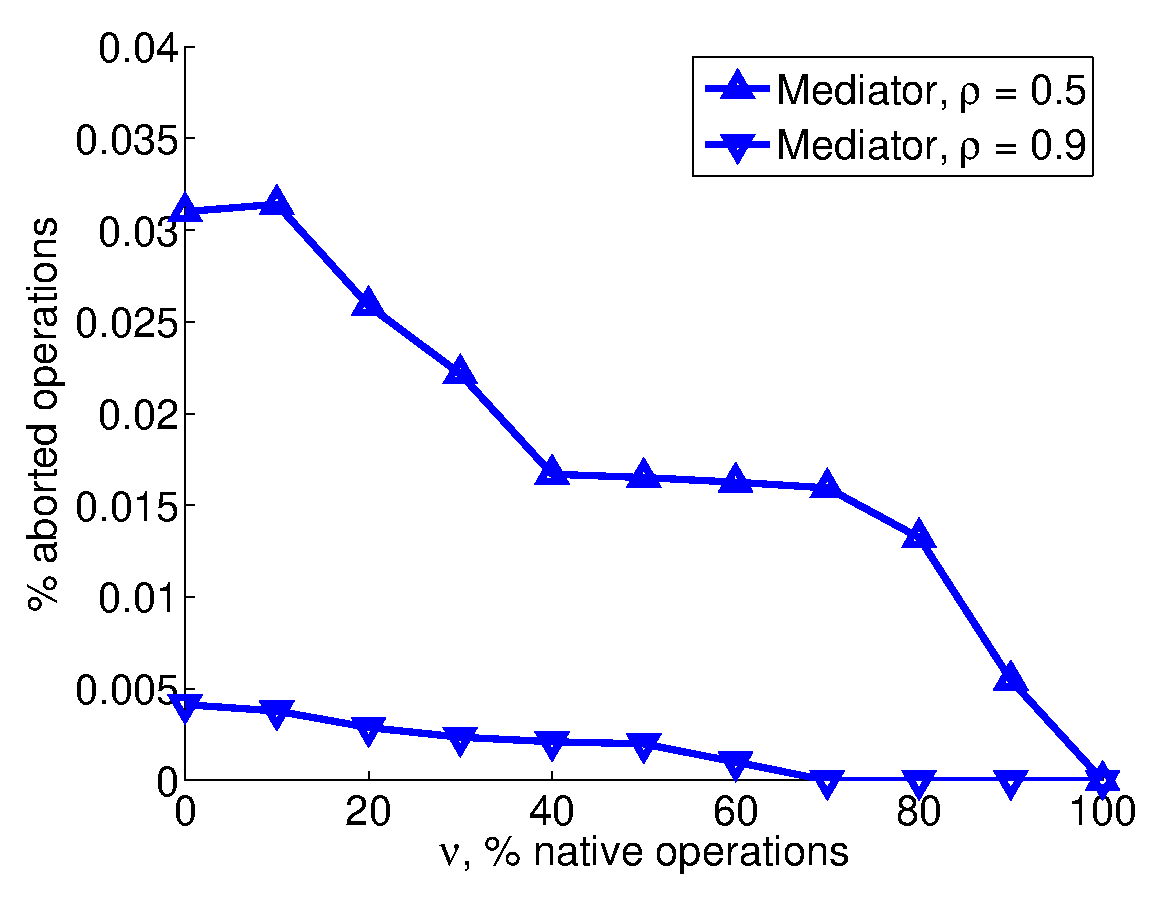
\includegraphics[width=2.5in]{Figs/matlab/abort_ratio_50r_u4.eps}
\caption{\bf{\small{Mediator's abort ratios, for the $\uniform{4}$ workload 
generated by $200$ clients ($0 \leq \nu \leq 1$, $\rho=0.5$ and $\rho=0.9$). 
For read-intensive workloads, the abort ratio is significantly smaller.}}}
\label{fig:abort_ratio}
%\vskip -.2.5in
\end{figure}
}


%\subsubsection{Scalability}
%\label{sec:eval:scalability}

{\bf Scalability.} Finally, we study Mediator's bottlenecks, to get an insight about its 
scalability limits. 
We take a closer look at the $\uniform{4}$ traffic pattern ($\rho=0.5, \nu=0$), 
for the number of clients $C$ ranging from $50$ to $500$. 
Figure~\ref{fig:latency_breakdown} depicts the latency breakdown 
by the time spent on significant internal API's. In this context, the datapath 
calls that happen upon commit (the native conflict check, the WAL, and the database 
write) account for over $70\%$ of transaction latency, whereas TSO's API's consume 
less than $20\%$. For very large numbers of clients, this fraction drops below 
$10\%$, which demonstrates that the TSO scales better than the database. 
The begin timestamp retrieval %$\medserver$.txTimestampRequest() call 
is a non-negligible component. This happens due to the oracle's state replication that 
is piggybacked on this request. 
%($\dbserver$.checkNativeConflicts(), $\logger$.append(), and $\dbserver$.txPut()) 
%($\medserver$.txTimestampRequest() and $\medserver$.txTryCommit()) 

%The database and the logger components are the system's bottlenecks, despite
% the fact that they are both distributed. 
The overhead of write-ahead logging might be reduced 
by employing state-of-the-art shared log services (e.g., Corfu~\cite{Corfu2012} 
uses specialized hardware, and boasts sub-millisecond latencies for loads similar 
to those exercised in our experiment). The potential upside 
of this optimization is approximately $25\%$ reduction of transaction latency.

\begin{figure}
\centering{
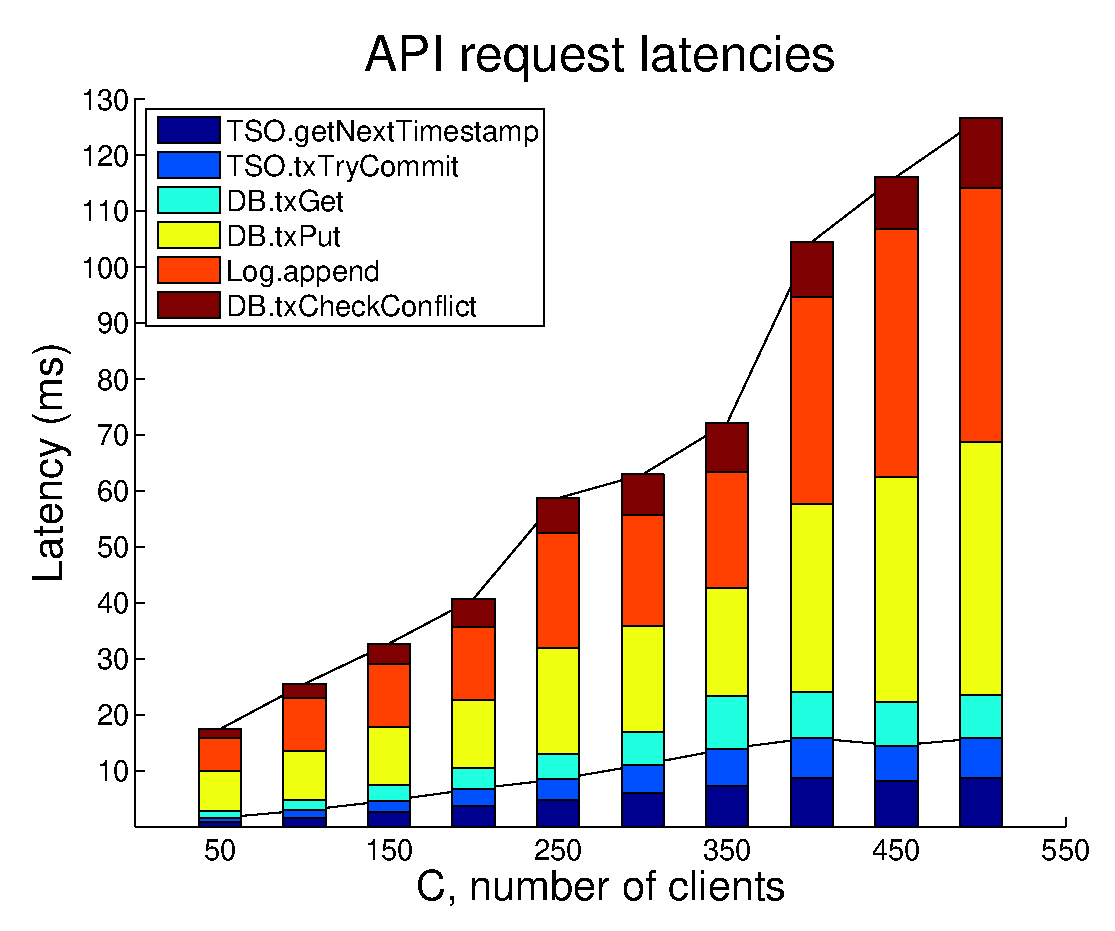
\includegraphics[width=2in]{Figs/matlab/latency_breakdown.eps}
}
\caption{\bf{\small{Breakdown of internal API request latencies, for the $\uniform{4}$ workload 
($\rho=0.5, \nu=0$), with a varying number of clients. The database and the 
logger layers are the execution bottlenecks.}}}
\label{fig:latency_breakdown}
%\vskip -.2.5in
\end{figure}


\subsection{Numerical Results -- Serializability}
\label{sec:tests:ser}

We conclude our experimentation by evaluating the overhead required to support
transaction serializability. In this setting, the algorithm incurs additional 
overhead (sending the transaction's read set to the TSO, in conjunction with the write set), 
and tests for read-write conflicts instead of write-write conflicts (Section~\ref{sec:ser}). 

We compare the serializability implementation's performance with the one for snapshot isolation,
by repeating the experiment in Section~\ref{sec:tests:si}, which evaluates Mediator with transaction-only 
traffic ($\nu=0$). 
%For singleton transactions ($\uniform{1}$), no difference exists, 
%since single-{\em get\/} transactions enjoy the no-commit optimization. 
%The results of comparison for the $\uniform{4}$ transaction size distribution 
%appear in Figure~\ref{fig:ser_comparison}. 
%
For read-dominated workloads ($\rho=0.9$), communication and
processing for serializability support incurs a significant overhead -- up to
$30\%$ less throughput in similar operating points. 
%As explained, this is due to sending all read sets to TSO instead of only 
%the write sets in snapshot isolation. Therefore, the communication and
% processing overheads are increased multiple times. 
%The impact is most pronounced with especially light loads. 
For write-intensive traffic ($\rho=0.5$), the performance gap is negligible. 
These results resonate well with other performance studies in the database 
literature~\cite{Alomari2008,Cahill2008}.


\remove{
\setlength{\abovecaptionskip}{9pt}
\setlength{\belowcaptionskip}{-11pt}
\begin{figure*}
  \centering
  \begin{subfigure}[b]{0.5\textwidth}
		{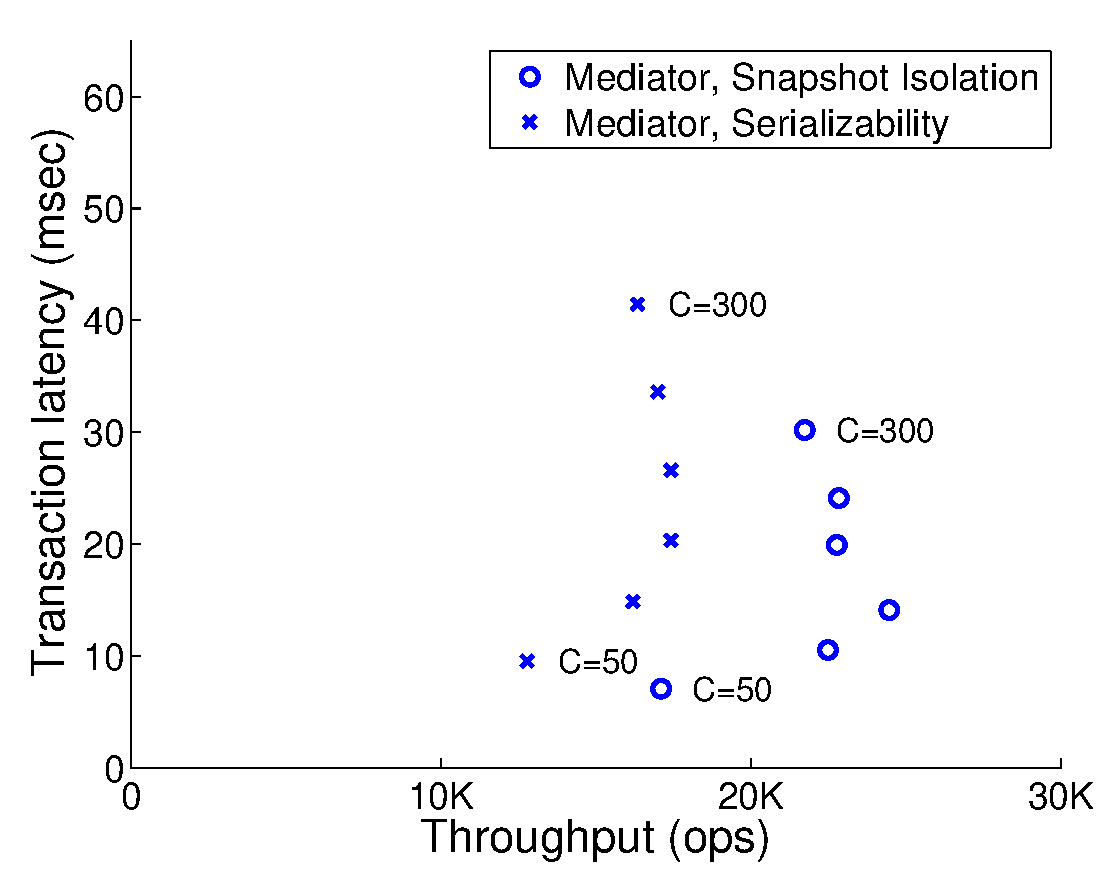
\includegraphics[width=2.5in]{Figs/matlab/throughput_latency_u4_90r_ser.eps}}
		\caption{Read-dominated workload ($\rho=0.9$)}
  \end{subfigure}%
%\hspace{0.4in}
	\begin{subfigure}[b]{0.5\textwidth}
{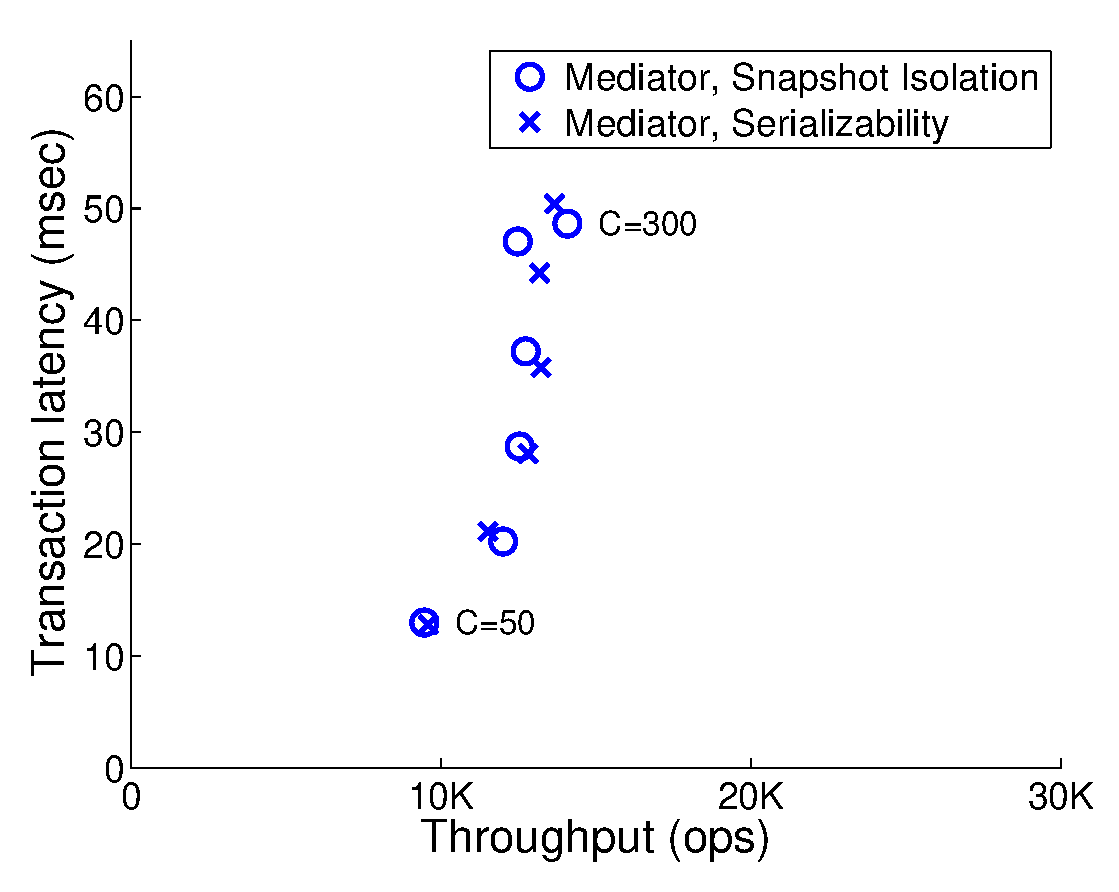
\includegraphics[width=2.5in]{Figs/matlab/throughput_latency_u4_50r_ser.eps}}
		\caption{Write-intensive workload ($\rho=0.5$)}
	\end{subfigure}

\caption{\bf{\small{Evaluation of the performance overhead incurred by supporting the serializability
consistency model. The Mediator implementations of snapshot isolation and serializability are 
compared for the $\uniform{4}$ transaction-only ($\nu=1$) traffic pattern, in the read-dominated 
($\rho=0.9$) and write-intensive ($\rho=0.5$) settings. The performance gap is substantial 
in the first case, and negligible in the second one. }}}
\label{fig:ser_comparison}
%\vskip -.2.5in
\end{figure*}
}